\documentclass{article}
\usepackage{blindtext}
\usepackage[T1]{fontenc}
\usepackage[polish]{babel}
\usepackage[utf8]{inputenc}
\usepackage{listings}
\usepackage{graphicx}
\usepackage{float}
\graphicspath{ {./Wykresy/} }

\title{Analiza wpływu zastosowania wybranych technik przygotowania danych do analizy, na jakość analizy danych}
\author{Dariusz Litwiński}
\date{\today}

\renewcommand\lstlistingname{Przykład}

\begin{document}
\maketitle
\section{Problem Analizy Danych}

\subsection{Analiza Danych}
Analiza danych to proces, w którym surowe dane są przekształcane w wiedzę i spostrzeżenia, na podstawie których można podejmować lepsze decyzje. []
Wewnątrz tego procesu można wyróżnić następujące fazy:
\subsubsection{Pozyskiwanie: gromadzenie danych}
Zanim analiza danych będzie możliwa należy pozyskać dane.
Dane mogą mieć różne źródła: czujniki, ankiety, 
Mogą być różnie przechowywane: pliki csv, bazy danych
\subsubsection{Przygotowanie: przetwarzanie danych}
Aby móc w pełni korzystać ze zgromadzonych danych, należy je przygotować: odpowiednio sformatować, wykorzystać techniki preprocessingu. To głównie tą częścią analizy danych będziemy się zajmować w dalszej części pracy. 
\subsubsection{Analiza: modelowanie danych}
Najczęsciej kiedy ktoś mówi "Analiza danych" to ma na myśli własnie tą część całego procesu, jakim jest Analiza Danych. To właśnie wykorzystywane są techniki trenowania sztucznej inteligencji, tworzone są klasyfikatory, które później możemy wykorzystywać do różnych zadań
\subsubsection{Działanie: podejmowanie decyzji}
Kiedy mamy już gotowe wyniki analizy, wtedy możemy je wykorzystać aby podjąć konkretne decyzje w prawdziwym świecie: Wykorzystać stworzony klasyfikator w diagnostyce chorób, 

\subsection{Problemy z Danymi}

Bardzo często zebrane dane nie nadają się bezpośrednio do pracy z nimi. Należy najpierw wykonać szereg operacji aby pozbyć się następujących problemów:   
\subsubsection{Brakujące wartości}
W danych mogą występować brakujące wartości, na przykład czujniki mogą różnić się między sobą ilością pobieranych parametrów, ankietowani mogą pozostawić niektóre pytania bez odpowiedzi. 
Brakujące wartości stanowią poważny problem, ponieważ model nie potrafi ich jednoznacznie zinterpretować, dlatego w trakcie przygotowania danych musimy podjąć decyzję, czy usunąć rekordy z brakującymi wartościami, 
przez co możemy znacznie zmniejszyć liczebność zbioru danych. Alternatywnym podejściem jest wypełnienie brakujących wartości. W miejsce braku może być wstawiona średnia, minimum, maksimum, lub też inna arbitralnie wybrana wartość. 
Pozornie wartości wstawiane w puste miejsca są kompletnie arbitralne, jednak bardzo często takie podejście skutkuje najlepszymi rezultatami, pod warunkiem że dobierzemy odpowiednią wartość do wstawiania. 
\subsubsection{Wartości odstające}
W niektórych przypadkach w danych mogą pojawić się takie wartości, 
które wyraźnie odstają od reszty i nie wnoszą sobą zbyt wiele informacji w kontekście analizy danych. 
Co więcej, mogą one zaciemniać pozostałą część danych, 
maskując trendy bądź prowadząc do błędnych wniosków. Dlatego najlepszym podejściem jest wykrywanie oraz usuwanie wartości, które możemy uznać za odstające. 
Istnieją algorytmy pozwalające nam na odrzucenie wartości odstających.
\subsubsection{Kolumny kategoryczne}
Wiele z modeli może pracować jedynie na wartościach liczbowych, podczas kiedy w zbiorach danych możemy znaleźć nie tylko takie wartości, ale również kategoryczne. Rezygnując z analizy tych danych tracilibyśmy wiedzę, jaką można z nich pozyskać. Nie jest to jednak konieczne, gdyż istnieją sposoby, aby zamienić te dane na postać liczbową za pomocą kodowania

\subsection{Znaczenie przygotowania danych}


\section{Metody Przygotowania Danych}
Istnieje kilka najczęściej używanych metod przygotowania danych, które dzielą się na następujące grupy:

\subsection{Uzupełnianie brakujących wartości}
Najczęściej brakujące wartości w zbiorach danych uzupełnia się średnią lub najczęściej występującą wartością, jednak może zdarzyć się tak, 
że najlepszym rozwiązaniem jest uzupełnienie braków minimum, maksimum, 
zerem bądź inną arbitralnie wybraną wartością
\subsection{Wykrywanie wartości odstających}
Do wykrywania wartości odstających możemy wykorzystać manualne metody, ale również i algorytmy, które wykryją te wartości za nas. 
Do manualnych metod możemy zaliczyć: Wykrywanie za pomocą rozkładu normalnego, Z-score, IQR, wykrywanie za pomocą percentyli. 
Natomiast spośród automatycznych metod mamy do dyspozycji między innymi Las Izolacji lub Local Outlier Factor
\subsection{Kodowanie wartości kategorycznych}
Jeżeli znamy zależności między klasami i możemy je uporządkować, wtedy jesteśmy w stanie dokonać kodowania ręcznie, na przykład najmniejszą wartość dla edukacji podstawowej, a najwyższą dla edukacji wyższej. Natomiast jeżeli nie znamy tych zależności, możemy wykorzystać LabelEncoder, jednak on ponumeruje klasy w kolejności alfabetycnzej, co nie zawsze jest pożądanym rezultatem. Innym podejściem jest One-Hot Encoding, który dla każdej z klas tworzy osobną kolumnę z wartością logiczną opisującą, czy dany rekord należy do tej klasy. Powoduje to wygenerowanie sporej ilości kolumn, jednak mamy wtedy pewność, że nie stworzymy nowych zależności między klasami
\subsection{Standaryzacja}
Standaryzacja jest procesem, po zakończeniu którego zmienna ma średnią wartość oczekiwaną zero oraz odchylenie standardowe równe jeden, 
dzięki czemu zyskujemy większą przejrzystość w jej analizie. Bardziej wyraźne są skupienia wokół konkretnych wartości, jednak należy zadbać o to, aby przed standaryzacją pozbyć się wartości odstających, gdyż będą one miały negatywny wpływ na zmienną po standaryzacji



\section{Środowisko wykonawcze}
\subsection{Specyfikacja sprzetowa, system i środowisko}
Sprzęt: Laptop wyposażony w procesor Intel Core i5-1135G7 (2.4Ghz) ze zintegrowaną grafiką oraz 16GB pamięci RAM
System operacyjny: Windows 10 Education
Menadżer środowisk: Anaconda Navigator
Python: 3.9.12
Edytor kodu: Visual Studio Code z dodatkami do edycji plików w formacie Jupyter notebook
\subsection{Zbiory danych}
Zbiory na których będziemy sprawdzać wpływ przygotowania danych są zbiorami do klasyfikacji. Do eksperymentów wybrano następujące zestawy danych:
\subsubsection{League of Legends stats}
Zbiór zawierający statystyki postaci z gry League of Legends z dwóch wersji obecnego sezonu (13.1 oraz 13.3)
\subsubsection{Australian Rain Forecast}
Zbiór zawiera codzienne obserwacje dotyczące pogody z różnych lokalizacji na terenie Australii
\subsubsection{Titanic Survival}
Jest to zestaw informacji na temat pasażerów Titanica oraz tego, czy udało im się przeżyć, na podstawie czego budujemy model, który próbuje przewidzieć na podstawie informacji które mu przekażemy, czy dana osoba przeżyła katastrofę

\section{Wykonane Eksperymenty}
Dla każdego z wybranych zbiorów danych przeprowadzono 
przygotowanie danych według ustalonego scenariusza, 
a także dodatkowego scenariusza w którym głównym celem było 
indywidualne podejście do zbioru oraz wyciągnięcie możliwie 
jak najwięcej informacji z dostępnych danych
\subsection{Brak Preprocessingu}
Pierwszy scenariusz, który w przyszłości 
będzie punktem odniesienia polegał na usunięciu rekordów, 
w których występowały jakiekolwiek brakujące wartości

\begin{lstlisting}[language=Python, caption={Brak przygotowania danych dla zbioru danych Titanic}, captionpos=b]
    def no_preprocessing(df,num):
        df_1 = df.copy()
        df_1 = remove_missing(df_1)
        y = df_1['Survived']
        df_1= drop_columns(df_1,categorical)
        df_1 = df_1.apply(pd.to_numeric)
        X = df_1
        X_train, X_test, y_train, y_test = train_test_split(
            X, y, test_size=0.1, random_state=42)
        score("Titanic",
            num,
            "No Preprocessing",
            X_train,y_train,X_test,y_test)
    \end{lstlisting}

\subsection{Wypełeninie brakujących wartości średnią}
Drugi scenariusz zakładał wypełnienie brakujących 
wartości średnią za pomocą metod biblioteki pandas 
fillna() oraz mean()

\begin{lstlisting}[language=Python, caption={Wypełnienie brakujących wartości średnią}, captionpos=b]
    def fill_missing_mean(df, work_columns):
        for col in work_columns:
            df[col] = df[col].fillna(df[col].mean())
        return df
\end{lstlisting}

\subsection{Wypełeninie brakujących wartości minimum}
Kolejny scenariusz zakładał wypełnienie brakujących 
wartości średnią za pomocą metod biblioteki pandas fillna() 
oraz min()

\begin{lstlisting}[language=Python, caption={Wypełnienie brakujących wartości minimum}, captionpos=b]
    def fill_missing_max(df, work_columns):
        for col in work_columns:
            df[col] = df[col].fillna(df[col].min())
        return df
\end{lstlisting}

\subsection{Wypełeninie brakujących wartości maksimum}
Czwarty scenariusz zakładał wypełnienie brakujących 
wartości średnią za pomocą metod biblioteki pandas 
fillna() oraz max()

\begin{lstlisting}[language=Python, caption={Wypełnienie brakujących wartości maksimum}, captionpos=b]
    def fill_missing_max(df, work_columns):
        for col in work_columns:
            df[col] = df[col].fillna(df[col].max())
        return df
\end{lstlisting}

\subsection{Wypełeninie brakujących wartości za pomocą regresji liniowej}
W tym scenariuszu wykorzystano pozostałe rekordy, 
aby przy pomocy regresji liniowej wygenerować 
brakujące wartości

\begin{lstlisting}[language=Python, caption={Wypełnienie brakujących wartości za pomocą regresji liniowej}, captionpos=b]
    def fill_missing_regression(df, numeric):    
        for col in numeric:
            df_num = df[numeric]
            test_data = df_num[df_num[col].isnull()]
            df_num = df_num.dropna()
            x_train = df_num.drop(col,axis=1)
            y_train = df_num[col]
            lr = LinearRegression()
            lr.fit(x_train,y_train)
            test_col = []
            for i in numeric:
                if(i != col):
                   test_col.append(i)
            x_test = test_data[test_col]
            x_test = fill_missing_mean(x_test,test_col)
            y_pred = lr.predict(x_test)
            test_data[col] = y_pred
            for i in test_data.index.values:
                df.at[i,col] = test_data.loc[i][col]
            return df
\end{lstlisting}

\subsection{Standaryzacja}
Dzięki StandardScaler z biblioteki sklearn dokonano 
standaryzacji kolumn liczbowych

\begin{lstlisting}[language=Python, caption={Standaryzacja kolumn liczbowych}, captionpos=b]
    def standardize(df, work_columns):
        standard_scaler = preprocessing.StandardScaler()
        for col in work_columns:
            values = df[col].values
            df_scaled = standard_scaler.fit_transform(
                values.reshape(-1, 1)) 
            df_scaled = pd.DataFrame(df_scaled)
            df[col] = df_scaled
        return df
\end{lstlisting}

\subsection{Standaryzacja oraz skalowanie do przedziału (0,1)}
Dzięki StandardScaler z biblioteki sklearn dokonano 
standaryzacji wraz ze skalowaniem do przedziału (0,1) 
kolumn liczbowych

\begin{lstlisting}[language=Python, caption={Skalowanie do przedziału (0,1)}, captionpos=b]
    def normalize(df, work_columns):
        min_max_scaler = preprocessing.MinMaxScaler()
        for col in work_columns:
            values = df[col].values
            df_scaled = min_max_scaler.fit_transform(values.reshape(-1, 1)) 
            df_scaled = pd.DataFrame(df_scaled)
            df[col] = df_scaled
        return df
\end{lstlisting}

\subsection{Skalowanie do przedziału (0,1) oraz usunięcie wartości odstających}
Poza skalowaniem z poprzedniego scenariusza, 
wykorzystano algorytm LocalOutlierFactor do usunięcia 
wartości odstających

\begin{lstlisting}[language=Python, caption={Usuwanie wartości odstających}, captionpos=b]
    def remove_outliers_lof(df,work_columns):
        df_temp = df
        df_temp = df_temp.loc[:, work_columns]
        clf = LocalOutlierFactor(n_neighbors=2)
        clf.fit(df_temp)
        y_pred_outliers = clf.fit_predict(df_temp)
        df_temp['outlier'] = y_pred_outliers

        df_temp = df_temp.loc[df_temp['outlier'] == 1]
        df_temp.drop('outlier', axis=1, inplace=True)
        df_temp = df_temp.reset_index(drop=True)
        df = df[df.index.isin(df_temp.index)]
        return df
\end{lstlisting}

\subsection{Kodowanie wartości kategorycznych}
Wykorzystano LabelEncoder z biblioteki sklearn do 
zakodowania wartości kategorycznych na liczbowe. 
W przypadku, kiedy dla danej kolumny brakowało wartości, 
rekord usuwano

\begin{lstlisting}[language=Python, caption={Usuwanie wartości odstających}, captionpos=b]
    def encode_categorical(df,work_columns):
        encoder = LabelEncoder()
        for col in work_columns:
            df[col] = encoder.fit_transform(df[col])
        return df
\end{lstlisting}

\subsection{Kodowanie wartości kategorycznych oraz wypełnienie brakujących wartości średnią}
Po wykonaniu kodowania z poprzedniego scenariusza, wypełniono brakujące wartości wartością średnią
\subsection{Scenariusz indywidualnego podejścia do zbioru danych}
\subsubsection{League of Legends stats}
Dla statystyk z gry League of Legends jedyne co mogło być zrobione poza operacjami z poprzednich scenariuszy było usunięcie kolumny z imieniem postaci, 
jako że nie wnosiła ona konkretnych informacji, a głównie identyfikowała dany rekord

\begin{lstlisting}[language=Python, caption={Indywidualny scenariusz dla zestawu danych LoL Stats}, captionpos=b]
    def custom_scenario(df,num):
        df_10 = df.copy()
        df_10 = fill_missing_mean(df_10,numeric)
        df_10 = remove_outliers_lof(df_10,numeric)
        df_10 = normalize(df_10,numeric)
        df_10= drop_columns(df_10,['Name'])
        df_10 = encode_categorical(df_10,to_be_encoded)
        y = df_10['Tier']
        df_10 = df_10.apply(pd.to_numeric)
        X = df_10
        X_train, X_test, y_train, y_test = train_test_split(
            X, y, test_size=0.1, random_state=42)
        score(
            "LoL_Stats",
            num,
            "Custom_preprocessing",
            X_train,y_train,X_test,y_test)
\end{lstlisting}

\subsubsection{Australian Rain Forecast}
Dla Australian Rain Forecast rozbito datę na dzień miesiąca, miesiąc oraz rok, 
dzięki czemu w teorii możemy zaobserwować trendy dotyczące na przykład poszczególnych miesięcy na przestrzeni wielu lat

\begin{lstlisting}[language=Python, caption={Indywidualny scenariusz dla zestawu danych Aus Weather}, captionpos=b]
    def custom_scenario(df,num):
        df_10 = df.copy()
        df_10 = fill_missing_mean(df_10,numeric)
        df_10 = remove_outliers_lof(df_10,numeric)
        df_10 = normalize(df_10,numeric)
    # Extract day, month and year from date
        df_10['Year'] = pd.DatetimeIndex(df_10['Date']).year
        df_10['Month'] = pd.DatetimeIndex(df_10['Date']).month
        df_10['Day'] = pd.DatetimeIndex(df_10['Date']).day
        df_10= drop_columns(df_10,['Date'])
        to_be_encoded = [
            'Location',
            'WindGustDir',
            'WindDir9am',
            'WindDir3pm',
            'RainToday',
            'Day',
            'Month',
            'Year']
        df_10 = encode_categorical(df_10,to_be_encoded)
        y = df_10['RainTomorrow']
        df_10 = df_10.apply(pd.to_numeric)
        X = df_10
        X_train, X_test, y_train, y_test = train_test_split(
            X, y, test_size=0.1, random_state=42)
        score(
            "Aus_weather",num,"Custom_preprocessing",
            X_train,y_train,X_test,y_test)
\end{lstlisting}

\subsubsection{Titanic Survival}
Dla zestawu danych Titanic wyciągnięto informację o tytule, jakim posługiwał się dany pasażer, 
dzięki czemu uzyskaliśmy informację o grupie społecznej, 
do której należeli pasażerowie. Dokonano również zmiany informacji o kabinie, którą zajmował pasażer, 
znacznie cenniejszą informacją od konkretnej kabiny jest sektor, w którym ona się znajdowała, 
informacja ta została uzyskana poprzez ograniczenie kodu kabiny jedynie do pierwszego znaku, który określa sektor

\begin{lstlisting}[language=Python, caption={Usuwanie wartości odstających}, captionpos=b]
    def custom_scenario(df,num):
        df_10 = df.copy()
        df_10['Title'] = df_10['Name'].str.extract(
            ' ([A-Za-z]+)\.', expand=False)
        df_10['Title'] = df_10['Title'].fillna(
            df_10['Title'].mode().iloc[0])
        df_10['Title'] = df_10['Title'].replace([
            'Lady', 'Countess','Capt', 'Col','Don', 'Dr',\
            'Major', 'Rev', 'Sir', 'Jonkheer', 'Dona'], 'Rare')
        df_10['Title'] = df_10['Title'].replace('Mlle', 'Miss')
        df_10['Title'] = df_10['Title'].replace('Ms', 'Miss')
        df_10['Title'] = df_10['Title'].replace('Mme', 'Mrs')
        df_10 = df_10.drop(['Name','Ticket','PassengerId'],axis=1)
        df_10['Cabin'] = df_10['Cabin'].fillna('000')
        df_10['Cabin'] = df_10['Cabin'].str[:1]
        df_10 = fill_missing_mean(df_10,numeric)
        df_10 = df_10.fillna(df_10.mode().iloc[0])
        to_be_encoded = ["Sex","Embarked","Cabin","Title"]
        df_10 = encode_categorical(df_10,to_be_encoded)
        y = df_10['Survived']
        df_10 = df_10.apply(pd.to_numeric)
        X = df_10
        X_train, X_test, y_train, y_test = train_test_split(
            X, y, test_size=0.1, random_state=42)
        score(
            "Titanic",num,"Custom_preprocessing",
            X_train,y_train,X_test,y_test)
\end{lstlisting}

\section{Wyniki Eksperymentów}
\subsection{League of Legends stats}
\begin{figure}[H]
\centerline{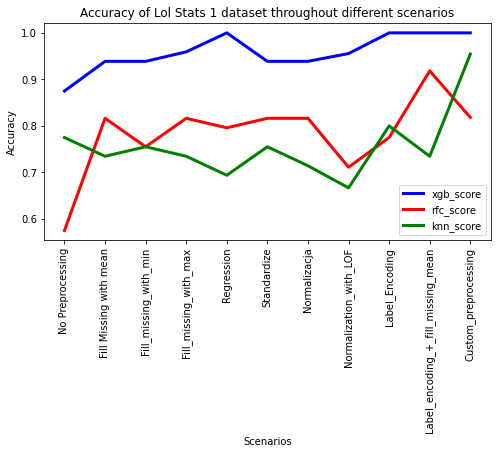
\includegraphics{Lol_Stats_1}}
\centering
\caption{Trafność klasyfikatorów po przygotowaniu danych według danego scenariusza}

\end{figure}

\begin{figure}[H]
\centerline{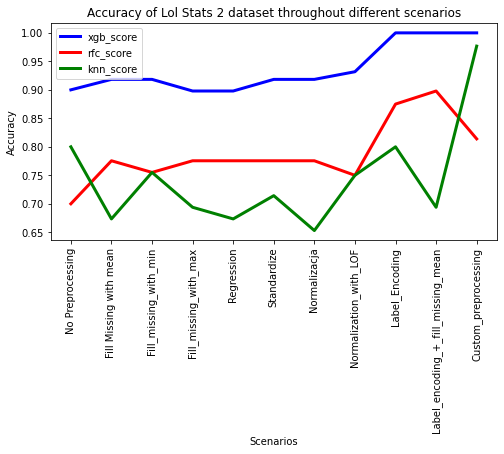
\includegraphics{Lol_Stats_2}}
\centering
\caption{Trafność klasyfikatorów po przygotowaniu danych według danego scenariusza}
\end{figure}

\begin{figure}[H]
\centerline{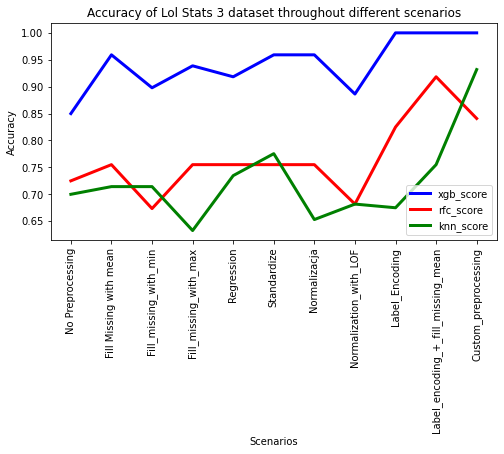
\includegraphics{Lol_Stats_3}}
\centering
\caption{Trafność klasyfikatorów po przygotowaniu danych według danego scenariusza}
\end{figure}

\subsection{Australian Rain Forecast}

\begin{figure}[H]
\centerline{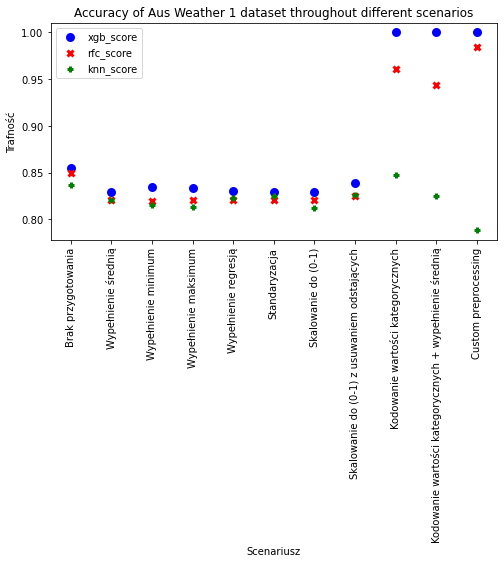
\includegraphics{Aus_Weather_1}}
\centering
\caption{Trafność klasyfikatorów po przygotowaniu danych według danego scenariusza}
\end{figure}
    
\begin{figure}[H]
\centerline{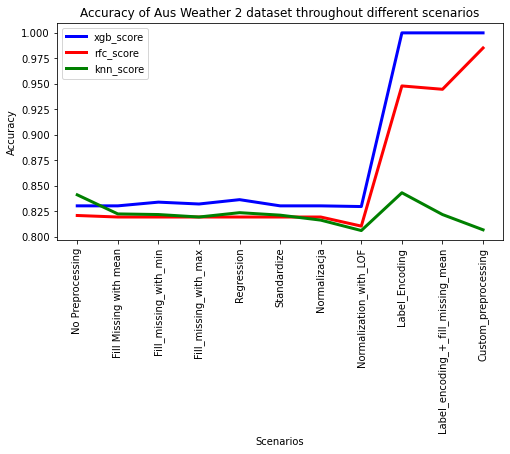
\includegraphics{Aus_Weather_2}}
\centering
\caption{Trafność klasyfikatorów po przygotowaniu danych według danego scenariusza}
\end{figure}
    
\begin{figure}[H]
\centerline{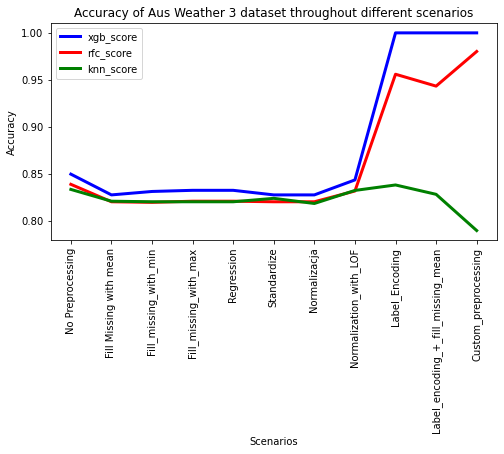
\includegraphics{Aus_Weather_3}}
\centering
\caption{Trafność klasyfikatorów po przygotowaniu danych według danego scenariusza}
\end{figure}


\subsection{Titanic Survival}

\begin{figure}[H]
\centerline{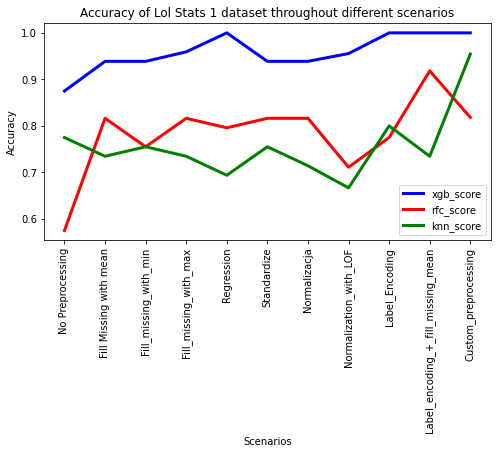
\includegraphics{Lol_Stats_1}}
\centering
\caption{Trafność klasyfikatorów po przygotowaniu danych według danego scenariusza}
\end{figure}
        
\begin{figure}[H]
\centerline{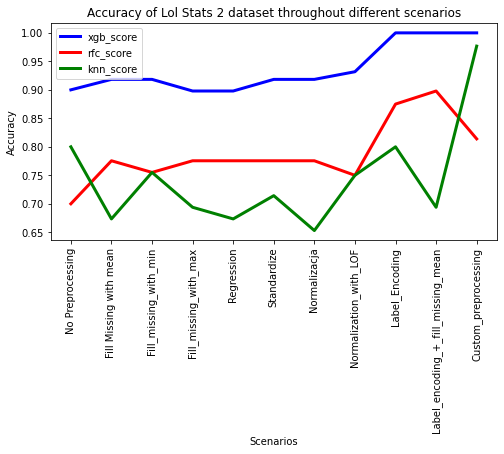
\includegraphics{Lol_Stats_2}}
\centering
\caption{Trafność klasyfikatorów po przygotowaniu danych według danego scenariusza}
\end{figure}
        
\begin{figure}[H]
\centerline{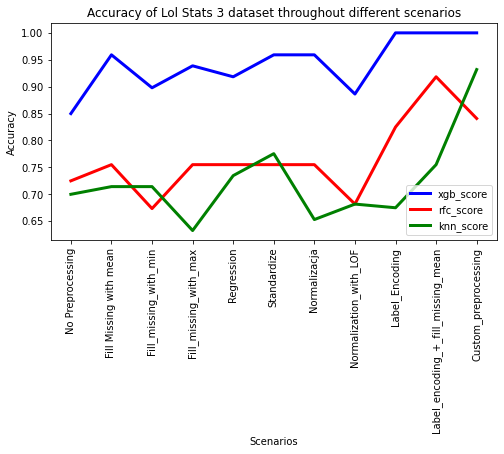
\includegraphics{Lol_Stats_3}}
\centering
\caption{Trafność klasyfikatorów po przygotowaniu danych według danego scenariusza}
\end{figure}
    
\subsection{Średnie wyniki}

\begin{figure}[H]
\centerline{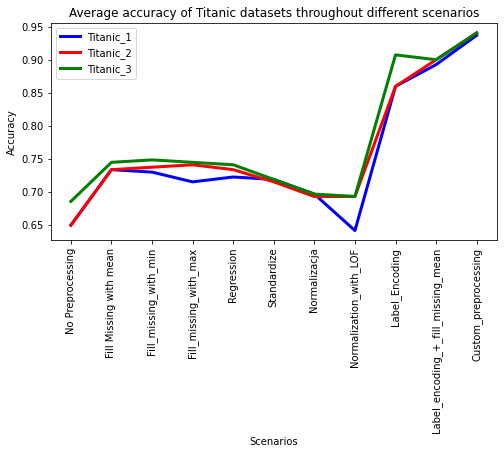
\includegraphics{Titanic_Avg}}
\centering
\caption{Średnia trafność klasyfikatorów po przygotowaniu danych według danego scenariusza}
\end{figure}
            
\begin{figure}[H]
\centerline{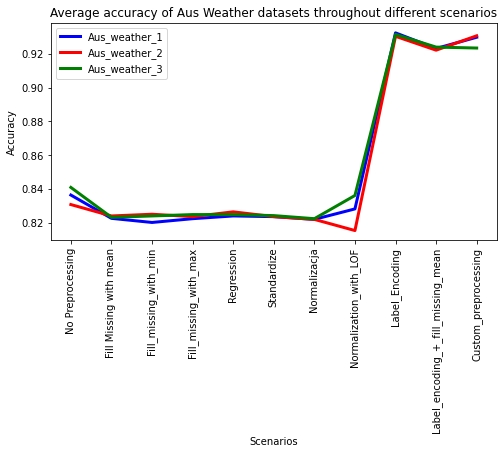
\includegraphics{Aus_Weather_Avg}}
\centering
\caption{Średnia trafność klasyfikatorów po przygotowaniu danych według danego scenariusza}
\end{figure}
            
\begin{figure}[H]
\centerline{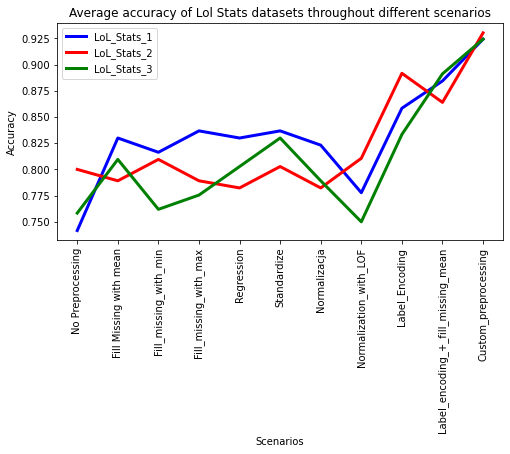
\includegraphics{Lol_Stats_Avg}}
\centering
\caption{Średnia trafność klasyfikatorów po przygotowaniu danych według danego scenariusza}
\end{figure}

\section{Podsumowanie}
Z przeprowadzonych eksperymentów wynika, 
że odpowiednie przygotowanie danych zwiększa trafność 
klasyfikatorów. Należy jednak zwrócić uwagę, że nie wszystkie 
scenariusze skutkowały jednoznaczną poprawą rezultatów. 
Na szczególne wyróżenienie zasługuje kodowanie wartości kategorycznych 
na liczbowe, gdyż w każdym przypadku zastosowanie tej metody znacznie zwiększyło
trafność klasyfikacji


\end{document}